\section{Régression linéaire avec une variable}
\subsection{Affichage des données}

Une pemière fonction \textit{plotData()}, qui permet d'afficher le profit du food truck en fonction de sa population sous forme de point. \\
L'objectif de cette partie sera de prédire le profit d'un food truck dans une nouvelle ville grâce à une descente de gradient en comprenant sa méthodologie.

\begin{figure}[!h]
    \begin{minipage}{.48\linewidth}
\begin{minted}[frame=lines, framesep=2mm, baselinestretch=1.2, fontsize=\footnotesize, linenos, breaklines=true]{python}
def plotData(X,y):
    fig = plt.figure()
    plt.plot(X, y, 'rx')
    plt.grid(True)
    plt.ylabel("Profit in $10,000s")
    plt.xlabel("Population of City in 10,000s")
    fig.show()
\end{minted}   
\captionof{listing}{Fonction plotData}
    \end{minipage}\hfill
    \begin{minipage}{.48\linewidth}
        \begin{center}
            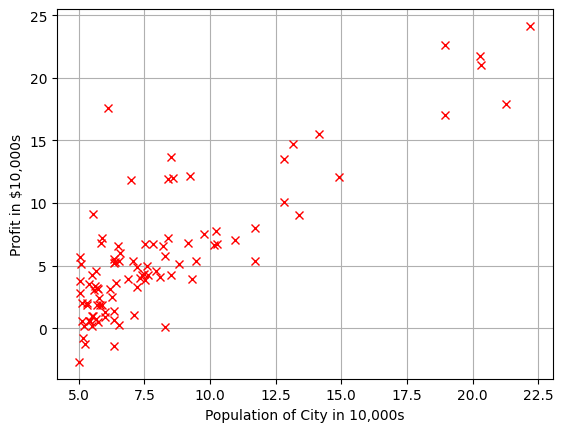
\includegraphics[width=1\textwidth]{./img/4-1.png}
            \caption{\label{fig:fig1}Profit en fonction de la population}  
        \end{center}
    \end{minipage}
\end{figure}

\subsection{Descente de gradient}

Le modèle de régression linéaire est représenté par l'équation \ref{eq:regression_linear}. Cette équation nous permet d'obtenir une prédiction en fonction d'une entré $x_1$ et de $\theta$.

\begin{equation}\label{eq:regression_linear}
    h_\theta(x) = x^T \theta =\theta_0 + \theta_1 x_1
\end{equation}

\noindent
Pour que cette prédiction soit optimal, il est important de déterminer correctement les paramètres de notre modèle: $\theta$. Pour cela, nous devons réaliser deux étapes: Le calcul du coût $J(\theta)$ et une descente de gradient.
    
\subsubsection{Calcul du coût $J(\theta)$}
Le calcul du coût $J(\theta)$ permet de mesurer la qualité de la prédiction, si le coût est faible alors notre prédiction est proche des valeurs réel et inversement si le coût est important.

\begin{equation}\label{eq:cout}
   J(\theta) = \underbrace{\frac{1}{2m} \sum_{i=0}^{m-1}}_{(b)}(\underbrace{h_\theta(x^{(i)}) - y^{(i)}}_{\text{(a)}})^2
\end{equation}

\begin{itemize}
    \item [(a)] \textbf{Différence entre la prédiction et la valeurs réel}, ce qui revient à déterminer l'erreur de la prédiction. On éléve le résultat au carré pour obtenir que des erreurs positives.
    \item [(b)] \textbf{Moyenne des erreurs}, ce qui nous permet d'obtenir le coût $J(\theta)$
\end{itemize}

\vspace{.3cm}

On remarque ici avec l'équation \ref{eq:cout} qui utilise l'équation \ref{eq:regression_linear}, que la seul valeur qui puisse influencer notre coût est $\theta$. Effectivement, les valeurs restante : $x$, $y$ et $m$; sont les valeurs
de notre problèmes qui sont déterminé et non modifiable.


\vspace{.5cm}
\noindent
\textbf{Mise en application}
\vspace{.2cm}


\begin{figure}[!h]
    \begin{minipage}{.48\linewidth}
\begin{minted}[frame=lines, framesep=2mm, baselinestretch=1.2, fontsize=\footnotesize, linenos, breaklines=true]{python}
def computeCost(X, y, theta):  
    m = y.size
    J = 0

    for i in range(0, m):
        J += (1/(2*m)) * (X[i].T @ theta - y[i])**2

    return J
\end{minted}   
\captionof{listing}{Fonction computeCost}
    \end{minipage}\hfill
    \begin{minipage}{.48\linewidth}
\begin{minted}[frame=lines, framesep=2mm, baselinestretch=1.2, fontsize=\footnotesize, breaklines=true]{text}
With theta = [0 ; 0] Cost computed = 32.0727 
Expected cost value (approx) 32.07

 -------------------------- 

With theta = [-1 ; 2] Cost computed = 54.242455
Expected cost value (approx) 54.24
\end{minted}   
\captionof{listing}{Output fonction computeCost}
    \end{minipage}
\end{figure}

Suite à la mise en application on constate effectivement l'influence de $\theta$ sur notre coût, on en déduit facilement qu'il est nécessaire de trouver la bonne valeur de $\theta$ pour minimiser ce coût. C'est le rôle de la descente de gradient.



\subsubsection{Descente de gradient}

La descente de gradient permet de minimiser le coût et donc d'obtenir les bonnes valeurs de theta pour réaliser une prédiction optimal.

\begin{equation}\label{eq:cout}
    \theta_j \coloneqq \theta_j - \alpha \frac{1}{m} \sum_{i=0}^{m-1} (h_\theta(x^{(i)}) - y^{(i)}) x_j^{(i)}
 \end{equation}

Pour mener à bien la descente de gradient on réalise à nouveau la moyenne des erreurs de prédiction mais cette fois-ci on la multiplie par un pas d'apprentissage $\alpha$. Ce pas permet de déterminer le taux d'apprentissage du modèle, 
plus il est grand plus l'apprentissage sera rapide, mais si ce taux est trop important alors la descente de gradient peut divergé d'un minimum. Il est donc important de choisir correctement ce pas. Ce gradient de la fonction de coût est ensuite
soustrait aux $\theta_j$ simulanément. \\
Il faut réaliser cette étape un certains nombres d'itérations pour converger vers un minimum.

\clearpage

\vspace{.5cm}
\noindent
\textbf{Mise en application}
\vspace{.2cm}

\begin{figure}[!h]
\begin{minted}[frame=lines, framesep=2mm, baselinestretch=1.2, fontsize=\footnotesize, linenos, breaklines=true]{python}
def gradientDescent(X, y, theta, alpha, num_iters):  
    m = y.size  # number of training examples
    n = theta.size # number of parameters
    cost_history = np.zeros(num_iters) # cost over iters
    theta_history = np.zeros((n,num_iters)) # theta over iters

    for n_iter in range(num_iters):
        for j in range(n):
            res = 0
            for i in range(m):
                res += (X[i].T @ theta - y[i]) * X[i][j]
            
            theta[j] = theta[j] - alpha * (1/m) * res

        cost_history[n_iter] = computeCost(X, y, theta)
        theta_history[:,n_iter] = theta.reshape((2,))
    
    return theta, cost_history, theta_history
\end{minted}   
\captionof{listing}{Fonction gradientDescent}\label{listing:gradient_descente}
\end{figure}

Après application de la fonction \ref{listing:gradient_descente} on obtient les résultats du listing \ref{listing:output_gradientDescent} et figure \ref{fig:fig2}, ce qui nous permet de conclure que nos valeurs de $\theta$ sont correct et que l'on à un modèle satisfaisant pour 
réaliser des prédictions optimal.

\begin{figure}[!h]
    \begin{minipage}{.48\linewidth}
\begin{minted}[frame=lines, framesep=2mm, baselinestretch=1.2, fontsize=\footnotesize, linenos, breaklines=true]{text}
Theta found by gradient descent: 
-3.6360634754795016 1.1669891581648786
Expected theta values (approx)
 -3.6303  1.1664
\end{minted}   
\captionof{listing}{Output fonction gradientDescent} \label{listing:output_gradientDescent}
    \end{minipage}\hfill
    \begin{minipage}{.48\linewidth}
        \begin{center}
            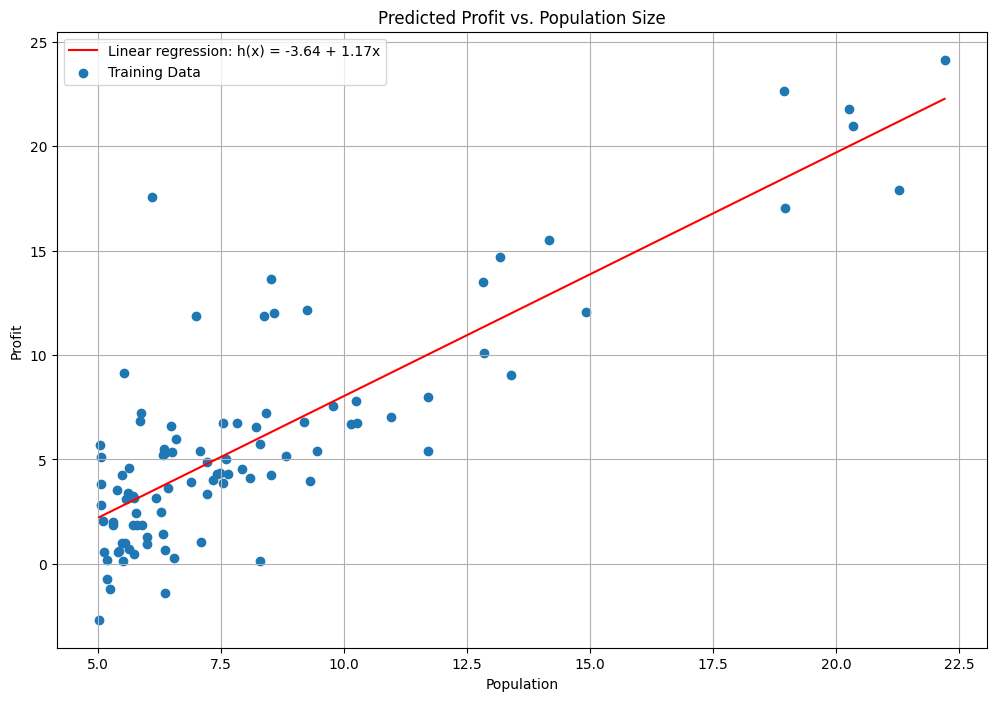
\includegraphics[width=1\textwidth]{./img/4-2-4(2).png}
            \caption{\label{fig:fig2}Profit prédit vs population}  
        \end{center}
    \end{minipage}
\end{figure}

\begin{figure}[!h]
\begin{minted}[frame=lines, framesep=2mm, baselinestretch=1.2, fontsize=\footnotesize, linenos, breaklines=true]{text}
For population = 35,000, we predict a profit of 4483.9858
For population = 70,000, we predict a profit of 45328.6063
\end{minted}   
\captionof{listing}{Prédiction}\label{listing:prediction1}
\end{figure}

\clearpage

\subsection{Visualisation de $J(\theta)$}


\begin{figure}[!h]
    \begin{center}
        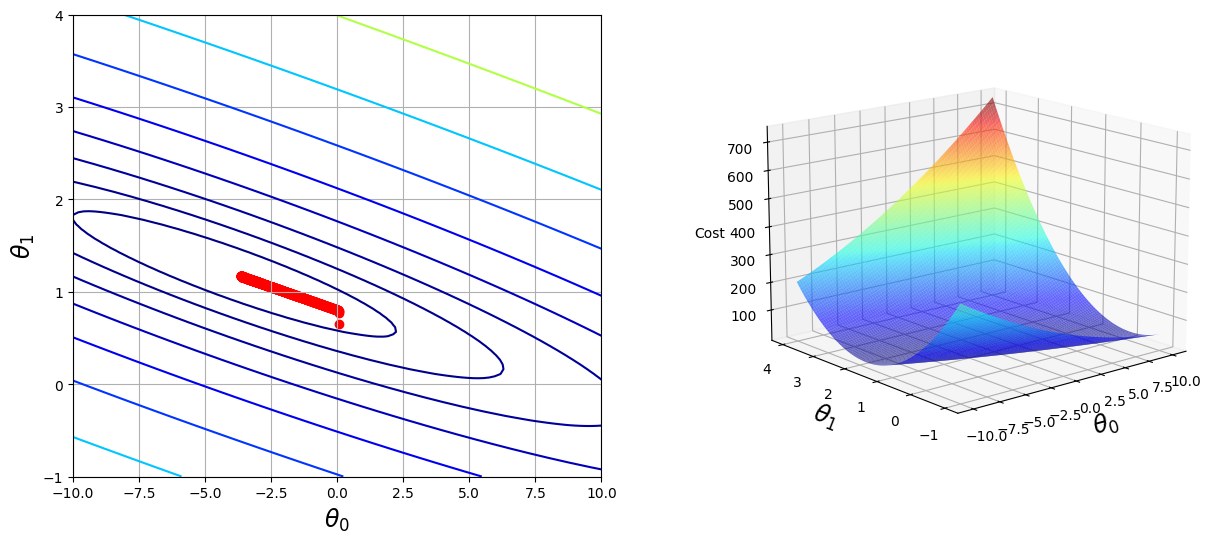
\includegraphics[width=1\textwidth]{./img/4-3.png}
        \caption{\label{fig:fig3}Visualisation de $J(\theta)$}  
    \end{center}
\end{figure}

Ce graphique nous permet de visualiser plus facilement de comment le coût $J(\theta)$ évolue, on remarque que les valeurs de $\theta$ sont modifié au fur est à mesure pour converger vers le centre de l'eclipse qui représente
le minimum optimal.
